% !TEX program = xelatex
\documentclass[a4paper,12pt]{article}

% --- Fonts & Japanese (XeLaTeX) ---
\usepackage{fontspec}
\usepackage{xeCJK}
\setmainfont[Scale=1.0,AutoFakeBold=2.0,AutoFakeSlant=0.2]{MS Mincho}
\setsansfont[Scale=1.0,AutoFakeBold=2.0,AutoFakeSlant=0.2]{MS Mincho}
\setmonofont[Scale=1.0,AutoFakeBold=2.0,AutoFakeSlant=0.2]{MS Mincho}
\setCJKmainfont[Scale=1.0,AutoFakeBold=2.0,AutoFakeSlant=0.2]{MS Mincho}
\setCJKmonofont[Scale=1.0,AutoFakeBold=2.0,AutoFakeSlant=0.2]{MS Mincho}

% --- Layout & readability ---
\usepackage[margin=25mm]{geometry}
\usepackage{setspace}
\setstretch{1.2}
\setlength{\parskip}{0.6em}
\setlength{\parindent}{1em}

% --- Math & symbols ---
\usepackage{amsmath,amssymb,bm}
\DeclareMathOperator{\stopgrad}{stopgrad}

% --- Graphics & color ---
\usepackage{graphicx}
\usepackage[dvipsnames]{xcolor}
\usepackage{float}

% --- Code/Pseudocode listings ---
\usepackage{listings}
\lstset{
  basicstyle=\ttfamily\small,
  columns=fullflexible,
  numbers=none,
  frame=single,
  framerule=0.3pt,
  rulecolor=\color{gray},
  breaklines=true,
  showstringspaces=false,
  xleftmargin=1em,
  framexleftmargin=1em,
  backgroundcolor=\color[gray]{0.98}
}

% --- Hyperref ---
\usepackage[unicode]{hyperref}
\usepackage[capitalize]{cleveref}
% 図・表ラベルの日本語化
\renewcommand{\figurename}{図}
% 日本語参照名(図/式)
\crefname{figure}{図}{図}
\Crefname{figure}{図}{図}
\crefname{equation}{式}{式}
\Crefname{equation}{式}{式}
\newtheorem{definition}{定義}
\hypersetup{
  colorlinks=true,
  linkcolor=blue,
  citecolor=blue,
  urlcolor=blue,
  pdfauthor={小笠 真治},
  pdftitle={LoRe: 不確実性ゲートで LLM の方策事前分布を安全に混合する},
}

% --- Bibliography (natbib numeric) ---
\usepackage[numbers,sort&compress]{natbib}
\bibliographystyle{unsrtnat}

\title{LoRe: 不確実性ゲートとKL制約によるLLM方策事前分布の安全混合 \\ \normalsize LoRe: Uncertainty-Gated, KL-Constrained Mixing of LLM Policy Priors in DreamerV3}
\author{小笠 真治\\香川高等専門学校}
\date{}
\renewcommand{\abstractname}{概要}

\begin{document}
\maketitle

\begin{abstract}
本稿は、モデルベース強化学習(MBRL)アルゴリズム DreamerV3 に対し、外部大規模言語モデル(LLM)の方策事前分布(policy prior)を必要なときだけ注入する軽量拡張 LoRe(Low-Regret LLM Prior)を提案する。LoRe の核は、(i) 状態依存の不確実性ゲートによる混合係数 $\beta(s)$、(ii) KL 逸脱のラグランジュ制御による安全側バイアス、(iii) API 予算・クールダウン・キャッシュによる実運用コスト抑制である。混合は単純なロジット加算
\begin{equation}\label{eq:mix}
\ell_{\mathrm{mix}}(s)=\ell_{\mathrm{wm}}(s)+\beta(s)\,\stopgrad\!\bigl(\tilde{\ell}_{\mathrm{llm}}(s)\bigr),\quad 
\pi_{\mathrm{mix}}=\mathrm{softmax}(\ell_{\mathrm{mix}})
\end{equation}
で実装され、LLM 側へは勾配を流さない。MiniGrid--DoorKey-5\,$\times$\,5 における早期スナップショット(約10k--12.7k steps)では、10k 近傍の成功率(SR)が RL のみ $\approx 0.025$ に対し LoRe $\approx 0.119$ と立ち上がりが早い。終盤 12.7k 近傍でも LoRe は $0.094$、RL のみは $0.021$ と上回った(Seed=42, GPU=cuda)。過剰混合は不安定化を招くため、$\beta$ と KL 目標の自動制御が有効である。DreamerV3 本体には改変を加えず、ロジット加算のみで統合できるため実装・計算コストは小さい\citep{hafner2023dreamerv3,minigrid_doorkey}。
\end{abstract}

\section{序論}
スパース報酬や手続き的依存をもつ環境では、初期探索の詰まりと行動の早期固定化が学習効率を阻害する。DreamerV3 は世界モデルによる想像訓練で多領域に通用するが、それでも初期段階の探索難は残ることがある。LLM は自然言語の手続き知識をもつため「鍵→ドア→ゴール」のような高次の順序構造に関するヒントを提供し得るが、常時参照は過依存と汎化劣化のリスクを伴う。LoRe は LLM を常時の操縦者ではなく不確実時の“助言者”として扱い、必要時のみ prior を混合して探索の端緒を促す設計である\citep{hafner2023dreamerv3,minigrid_doorkey}。本稿の貢献は三点に集約される。第一に、不確実性駆動の係数 $\beta(s)$ により状態依存に prior を混合する。第二に、混合による基底方策からの逸脱を KL 目標追従で安全側に抑制する。第三に、API 予算・クールダウン・キャッシュを備えた低侵襲の運用設計を示す。

\section{関連研究}
\textbf{Dreamer 系と環境系.} DreamerV3 は固定ハイパラで 150+ タスクを攻略する汎用 MBRL であり、本研究はその方策ヘッドに外部 prior を加える低侵襲拡張である。ベンチとして DoorKey(MiniGrid)はスパース報酬の古典的難題、Crafter/Craftax は探索・長期計画の能力を広く測る\citep{hafner2021crafter,matthews2024craftax}。

\textbf{LLM×行動/エージェント.} LLM を行動計画・実行に活用する流れは、Zero-Shot Planners(言語→行動列)\citep{huang2022lmp,huang2022pmlr}、ReAct(推論と行動の交互生成)\citep{yao2023react}、Voyager(Minecraft での自己拡張的スキル獲得)\citep{wang2023voyager}、Reflexion(言語による自己反省強化)\citep{shinn2023reflexion} 等により進展してきた。本研究は LLM を直接の行動者にせず、既存 RL 方策の prior として混合する点が異なる。評価系としては AgentBench/SmartPlay が整備されつつある\citep{liu2023agentbench,wu2023smartplay}。

\textbf{安全な混合・制約最適化.} KL 制約に基づく方策更新は TRPO、確率的推論としての RL 理論等により位置付けられており、LoRe の KL 逸脱制御はこの系譜にある\citep{schulman2015trpo,levine2018rlcontrol}。また探索における不確実性は、世界モデルの分岐不一致(disagreement)や価値分散、方策エントロピー等で測られてきた\citep{sekar2020plan2explore,pathak2019disagreement}。

\section{提案手法:LoRe}
\subsection{設計原則}
 LoRe は (a) 必要時のみ助言, (b) 基底方策からの逸脱抑制, (c) 実運用コスト抑制を同時に満たすことを目標とする。混合は加法ロジットで、DreamerV3 の学習則や損失の主構造に手を触れない。DreamerV3 実装や環境は既存リポジトリを参照する\citep{dreamerv3_github}。混合の中核は式\eqref{eq:mix}である。

 % (定義ボックスは削除)

\subsection{LLM 事前分布の温度整合}
LLM 側ロジットはスケールが異なるため、温度 $T_{\mathrm{temp}}>0$ を導入し
\begin{equation}\label{eq:temp}
\tilde{\ell}_{\mathrm{llm}}=\frac{\ell_{\mathrm{llm}}}{T_{\mathrm{temp}}},\qquad T_{\mathrm{temp}}=\arg\min_{t>0}\,\mathrm{KL}\!\left(\mathrm{softmax}\,\ell_{\mathrm{wm}}\,\middle\|\,\mathrm{softmax}\,\frac{\ell_{\mathrm{llm}}}{t}\right)
\end{equation}
とする。これは知識蒸留や確率校正の考え方に近い\citep{hinton2015distill,guo2017calibration}。

\subsection{不確実性ゲート $\beta(s)$}
方策エントロピー $\hat H[\pi_{\mathrm{wm}}]$、価値分散 $\widehat{\mathrm{Var}}[V]$、世界モデル分岐不一致 $\widehat{\mathrm{Dis}}$ を EMA 正規化し線形結合 $u(s)$ を作る。
\begin{equation}\label{eq:beta}
\beta(s)=\beta_{\max}\cdot \sigma\!\bigl(\kappa(u(s)-\tau)\bigr)
\end{equation}
高不確実な状態ほど prior を強める設計である\citep{sekar2020plan2explore,pathak2019disagreement}。

\subsection{KL 逸脱のラグランジュ制御}
混合方策と基底方策の乖離 $\mathrm{KL}(\pi_{\mathrm{mix}}\,\|\,\pi_{\mathrm{wm}})$ が目標 $\delta_{\mathrm{target}}$ を超えた分だけペナルティを課す:
\begin{equation}\label{eq:kl}
\mathcal{L}_{\mathrm{KL}}=\lambda\,\mathrm{ReLU}\bigl(\mathrm{KL}(\pi_{\mathrm{mix}}\,\|\,\pi_{\mathrm{wm}})-\delta_{\mathrm{target}}\bigr),
\end{equation}
\begin{equation}\label{eq:lambda}
\lambda \leftarrow \bigl[\,\lambda + \eta_\lambda\,\bigl(\mathrm{KL}(\pi_{\mathrm{mix}}\,\|\,\pi_{\mathrm{wm}})-\delta_{\mathrm{target}}\bigr)\,\bigr]_+.
\end{equation}

\section{実験設定}
\textbf{環境}: MiniGrid--DoorKey-5\,$\times$\,5(鍵取得→ドア解錠→ゴール、スパース報酬)。\textbf{評価指標}: 成功率(SR)。\textbf{学習ステップ}: 約 10k--12.7k の早期遷移を観察。\textbf{比較}: RL のみ vs LoRe($\beta$ ゲート+KL 制約+発火ポリシー有効)。DoorKey のタスク定義・難しさは公式ドキュメントを参照\citep{minigrid_doorkey}。

\section{結果}

\begin{figure}[H]
  \centering
  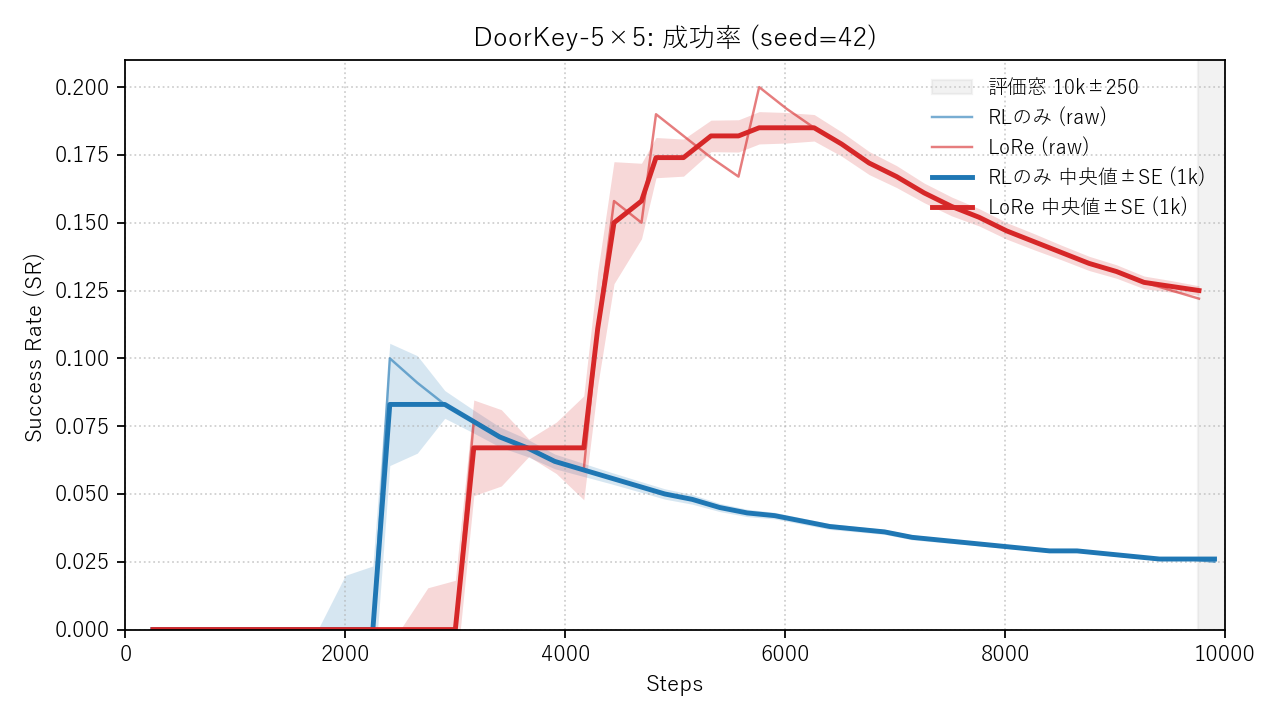
\includegraphics[width=\linewidth]{sr_compare.png}
  \caption{DoorKey-5\,$\times$\,5 における成功率(中央値±SE;評価窓=各1k steps;seed=42)。LoRe は6--10k域で一貫してRLのみを上回る。}
  \label{fig:sr}
\end{figure}

図\ref{fig:sr}は DoorKey-5\,$\times$\,5(seed=42)における SR の推移である。10k$\pm$250 steps の窓で算出した中央値は、RL のみが 0.025、LoRe が 0.119 であり、差分は +0.094 であった。時点比較でも、6k では LoRe=0.20 / RL=0.045、8k では 0.15 / 0.03、10k では 0.12 / 0.025 と、LoRe は中盤以降で一貫して優位である。LLM API の総発火は 98 回で、中盤(6--8k)に集中した。これらは、$\beta$ ゲート(式\eqref{eq:beta})により探索のボトルネックで prior が選択的に強まり、同時に KL 逸脱制御(式\eqref{eq:kl}, \eqref{eq:lambda})が過度な依存を抑制した結果と解釈できる。なお、本結果は単一 seed・早期スナップショットの観察であり、統計的検証には多 seed・長期学習が必要である。

\section{考察}
\textbf{効き所とメカニズム.} DoorKey のように明確な順序制約とスパース報酬がある課題では、LLM の手続き的知識は初期探索のボトルネックを緩和する。LoRe は不確実性が高い状態だけ prior を増やすため、LLM に全時刻を支配させず、DreamerV3 の学習ダイナミクス(想像訓練+価値学習)を大きく乱さない。これは、ロボティクスで LLM の高次知識と低次価値推定をゲートで統合する手法(SayCan)の着想とも親和的である\citep{ahn2022saycan}。

\textbf{制御の重要性.} 温度整合(式\eqref{eq:temp})がないと LLM ロジットは過鋭化し、方策が硬直しやすい。単一スカラーの温度 $T_{\mathrm{temp}}$ でスケールを合わせるだけでも安定性が向上する。さらに、KL のターゲットを緩→厳へとスケジューリングすれば、初期の探索支援と後期の自律収束を両立できる\citep{hinton2015distill,guo2017calibration}。

\textbf{位置付け.} ReAct/Voyager/Reflexion 等の「LLM を主体的エージェントとする」路線と比べ、LoRe は RL 方策主体+LLM は advisor という安全側の設計であり、既存 MBRL の再利用性が高い。将来的には AgentBench/SmartPlay など言語記述を伴う環境での prior 混合の汎化検証も有用だろう\citep{liu2023agentbench,wu2023smartplay}。

\section{アブレーション方針(今後の検証計画)}
(1) 温度整合 $T_{\mathrm{temp}}$ の有無/適応更新、(2) KL 目標 $\delta_{\mathrm{target}}$ のスケジューリング、(3) $\beta$ の構成要素(エントロピー・価値分散・分岐不一致)の寄与、(4) API 発火ポリシー(クールダウン・キャッシュ・マクロ境界)の有無、(5) 発火頻度の早期学習への寄与、などを追試する。探索の不確実性指標については Plan2Explore/Disagreement 系の測度設計も併用して比較する\citep{sekar2020plan2explore,pathak2019disagreement}。

\section{限界と今後の課題}
(i) 重み $w_H,w_V,w_D$ はタスク依存であり自動調整(メタ学習/ベイズ最適化)が望ましい。(ii) KL 目標の自動スケジュール(学習進行度指標に基づく適応)を導入したい。(iii) LLM からサブゴール列や高次表現のみを prior として渡し、視覚のドメインギャップに強い抽象度整合を図る設計も検討に値する。(iv) 本稿の結果は単一 seed の早期スナップショット比較であり、多 seed・長期学習・環境多様化で統計的検証を拡張する必要がある\citep{hafner2023dreamerv3}。

\section{再現性メモ}
リポジトリには、学習時に \texttt{src[wm,llm,rand]}, \texttt{prob\_max}, \texttt{entropy\_mix}, \texttt{KL(pi\_mix||pi\_wm)} をログ出力する。API 呼び出しはキャッシュ命中率とクールダウンを併記。障害時は、世界モデル再構成誤差、価値の過信、$\beta$ 飽和、KL 超過の恒常化をまず点検する。コードとディレクトリ構成は公開リポジトリを参照\citep{lore_github}。

\noindent\textbf{再現性の要約表}
\begin{center}
\begin{tabular}{ll}
環境ID & MiniGrid-DoorKey-5x5-v0 \\
乱数seed & 42 \\
学習総ステップ(ログ) & 20k steps \\
評価窓 & 各1k steps(中央値, SE) \\
評価時刻 & 6k/8k/10k,10k\,$\pm$\,250 \\
LLM API総発火(本ログ) & 98 回 \\
\end{tabular}
\end{center}

\section*{付録A:実装要約}
コード構成は \texttt{agents/}(DreamerV3: CNN+RSSM, actor-critic), \texttt{llm/}(温度整合・予算・キャッシュ), \texttt{trainers/}, \texttt{utils/}, \texttt{main.py}。ロギングは \texttt{src[wm,llm,rand]}、\texttt{entropy\_mix}、\texttt{KL(pi\_mix||pi\_wm)} などを出す。DreamerV3 の実装方針や環境セットアップは既存資源に準拠\citep{dreamerv3_github}。

\section*{付録B:記号表}
\begin{tabular}{ll}
$\ell_{\mathrm{wm}},\,\ell_{\mathrm{llm}}$ & 世界モデル/LLM のロジット\\
$\pi_{\mathrm{mix}}$ & 混合方策\\
$\beta(s)$ & 不確実性ゲート係数(式\eqref{eq:beta})\\
$T_{\mathrm{temp}}$ & 温度整合の温度(式\eqref{eq:temp})\\
$\delta_{\mathrm{target}}$ & KL 目標値\\
$\lambda$ & KL 罰のラグランジュ乗数(式\eqref{eq:lambda})\\
$\kappa,\,\tau$ & ゲートのスケール/しきい値\\
\end{tabular}

\section*{付録:学習ループ(高位擬似コード)}
混合はロジット加算、$\beta$ は不確実性ゲート、KL はラグランジュ制御。API は予算・クールダウン・キャッシュで節約。
\begin{lstlisting}[language=]
for step in range(T):
  logits_wm = actor_head(s)
  if allow_call(s):                      # 予算・クールダウン・キャッシュ・マクロ境界
    logits_llm = call_llm(s)
    T_temp = estimate_temperature(buffer)     # KL 最小化の1D探索
    u = uncertainty(s)                        # H[pi], Var[V], Disagreement の正規化結合
    beta = beta_max * sigmoid(k*(u - tau))
  else:
    logits_llm, beta = 0, 0

  logits_mix = logits_wm + stopgrad(beta * logits_llm / max(T_temp, eps))
  pi_mix = softmax(logits_mix)
  a ~ pi_mix
  s, r = env.step(a)

  update_world_model()
  kl = KL(pi_mix || softmax(logits_wm))
  loss_actor += lambda * relu(kl - delta_target)
  lambda = clip_pos(lambda + eta_lambda * (kl - delta_target))
\end{lstlisting}

% 参考文献の見出しを日本語に固定
\renewcommand{\refname}{参考文献}
\begingroup
\small
\bibliography{refs}
\endgroup

\end{document}
